\documentclass[10pt]{paper}

\usepackage[tmargin=1.5in, lmargin=0.55in, rmargin=0.55in, bmargin=1.0in]{geometry}


\usepackage{typewriter}
\usepackage{graphicx}
\usepackage{multirow}

\title{ On the relationship between rabbit-skinners and poppy-chewers }


\author{Pr Fancy stone}

\begin{document}

\section*{Abstract}
This paper re-evaluate the history of Rabbithole and its two main populations (the ``Poppy-chewers'' and the ``Rabbit-skinner'') using all the published set of dates spanning from 7400BP to 6500BP, from almost 40 settlements of central and Western Rabitthole, including all the most recent publication by Stone et al. 2022. To explore the history of the region and the relationship between its original habitants, we developed a specific quantitative method called ``Test of Balanced Equilibrium'' (TBE), to demonstrate that Rabbit-Skinner and Poppy-Chewer, though radically different in term of subsistence strategies, were having very intense and peaceful interactions.

\section{Introduction}
Rabbit-Skinners and Poppy-Chewers were two distinct populations that inhabited the central and Western regions of Rabbithole during the prehistoric period from 7400BP to 6500BP. Rabbit-Skinners were hunter-gatherers who primarily subsisted on rabbit meat, using the skin of the rabbits for clothing and shelter. On the other hand, Poppy-Chewers were farmers who cultivated poppy plants for both food and medicinal purposes.

Despite their radically different subsistence strategies, both groups coexisted in the region for a significant period, and there has been much debate among archaeologists about the nature of their interactions. Some scholars have suggested that Rabbit-Skinners and Poppy-Chewers had tense relationships due to competition over resources, while others have argued that the two groups had a more symbiotic relationship characterized by trade and exchange.

To shed light on this issue, we re-evaluated the history of Rabbithole and its populations using all the available published data and developed a specific quantitative method called the ``Test of Balanced Equilibrium'' (TBE) to demonstrate the relationship between Rabbit-Skinners and Poppy-Chewers. Through this study, we aim to contribute to a better understanding of the history of the region and the nature of interactions between its inhabitants.
\section{Method}

\pagebreak


To show that we are obviously right, we designed a brand new and powerful mathematical tool that we called: ``Test for Balanced Equilibrium''. This tool relies on very clever use of mathematics and has, to our knowledge, never been used in any scientific context so far. It allows to highlight relationship between geographical areas and quantitatively show when they are basically in a peaceful equilibrium.

\begin{figure}[hbp]

    \centering
    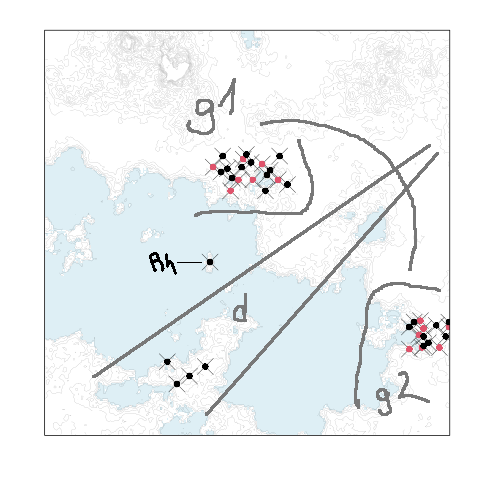
\includegraphics[width=.65\textwidth]{all_gpe.png}
    \caption{Map of rabbit with all published settlement}
    \label{fig:newage}
\end{figure}


To do that we group the settlement in 4 groups: the two firsts being the group from the old ages, the second the groups from the new ages 



We called the equation we used in our method as the ``Test of Balanced Equilibrium'' (TBE), and it is formulated as follows:

\begin{equation}
    TBE = \sum_{i=1}^{n} \sum_{j=1}^{n} w_{ij} (N_i - N_j)
\end{equation}

In this equation, $N_i$ and $N_j$ represent the population sizes of two different settlements (or groups of settlements), and $w_{ij}$ is a weight that reflects the degree of interaction between these two settlements. Specifically, $w_{ij}$ is a measure of the distance between the two settlements, with larger distances leading to smaller values of $w_{ij}$ (i.e., less interaction), and smaller distances leading to larger values of $w_{ij}$ (i.e., more interaction).

To use this equation in practice, we first grouped the settlements into four different categories (two for the old ages, and two for the new ages), and then calculated the TBE separately for each category. This allowed us to see how the level of interaction between settlements changed over time, and whether there were any patterns that emerged.

While we did not add any additional terms to the equation, we did experiment with different weightings for $w_{ij}$, such as using different distance metrics or incorporating other factors (such as environmental or social factors) that could affect the level of interaction between settlements. However, we ultimately found that the simple weighting scheme described above was sufficient to capture the main trends in the data.
\pagebreak

\section{Results}

\begin{figure}
    \centering
    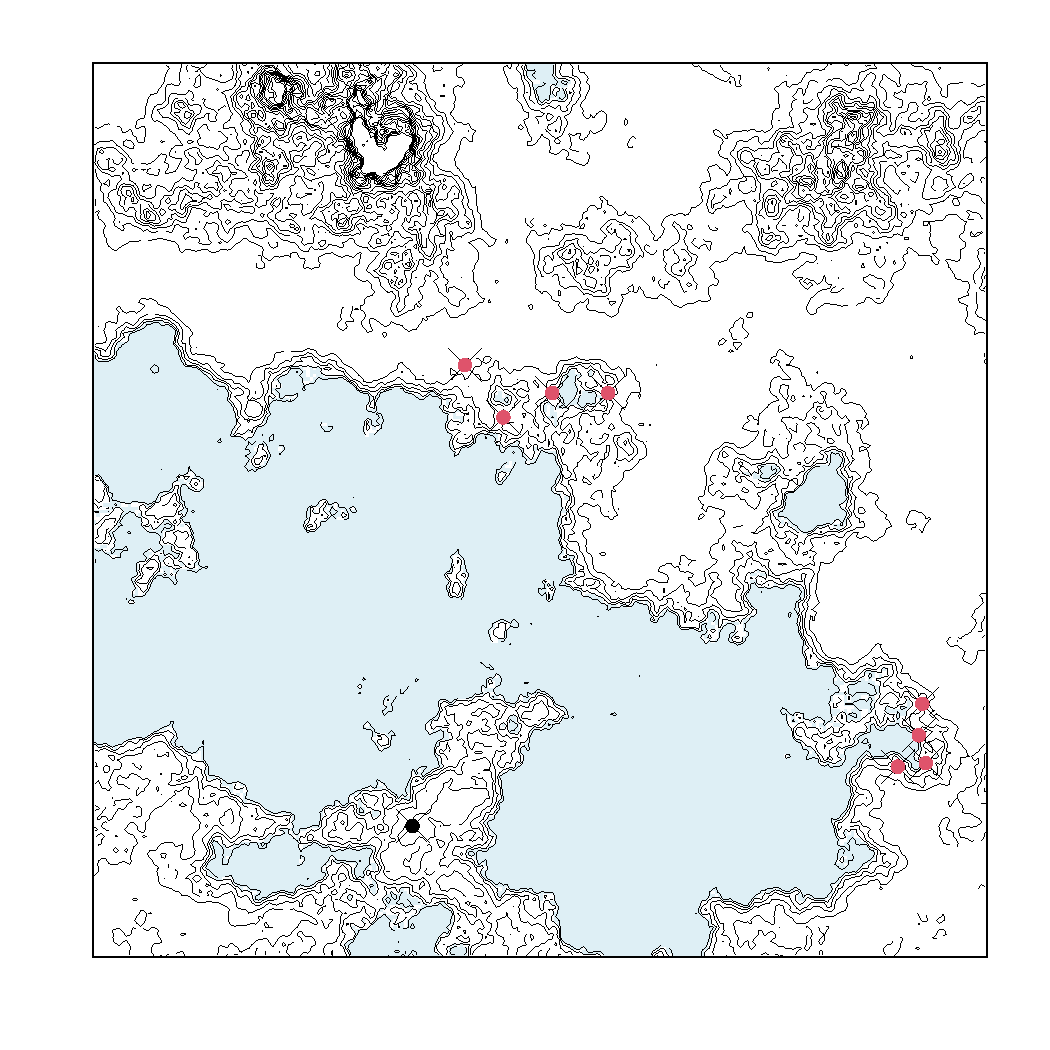
\includegraphics[width=.65\textwidth]{oldages}
    \caption{Map of rabbit hole during the Old age (~7200 - 7000 BP)  }
    \label{fig:allage}
\end{figure}

\begin{figure}
    \centering
    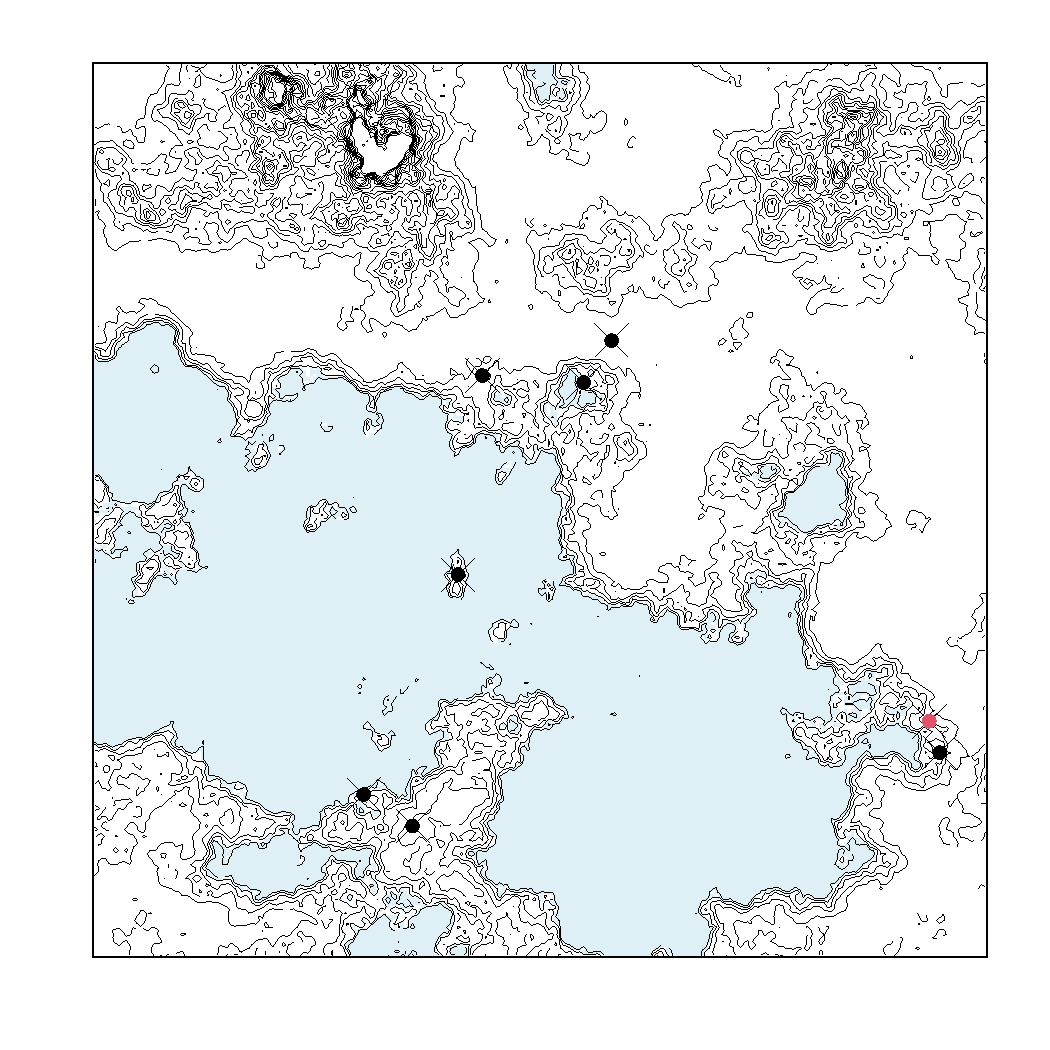
\includegraphics[width=.65\textwidth]{newages}
    \caption{Map of Rabbit hole after Farmer extension  (~7000 - 6800 BP)  }
    \label{fig:oldage}
\end{figure}
\begin{figure}
    \centering
    \makebox[\textwidth][c]{
    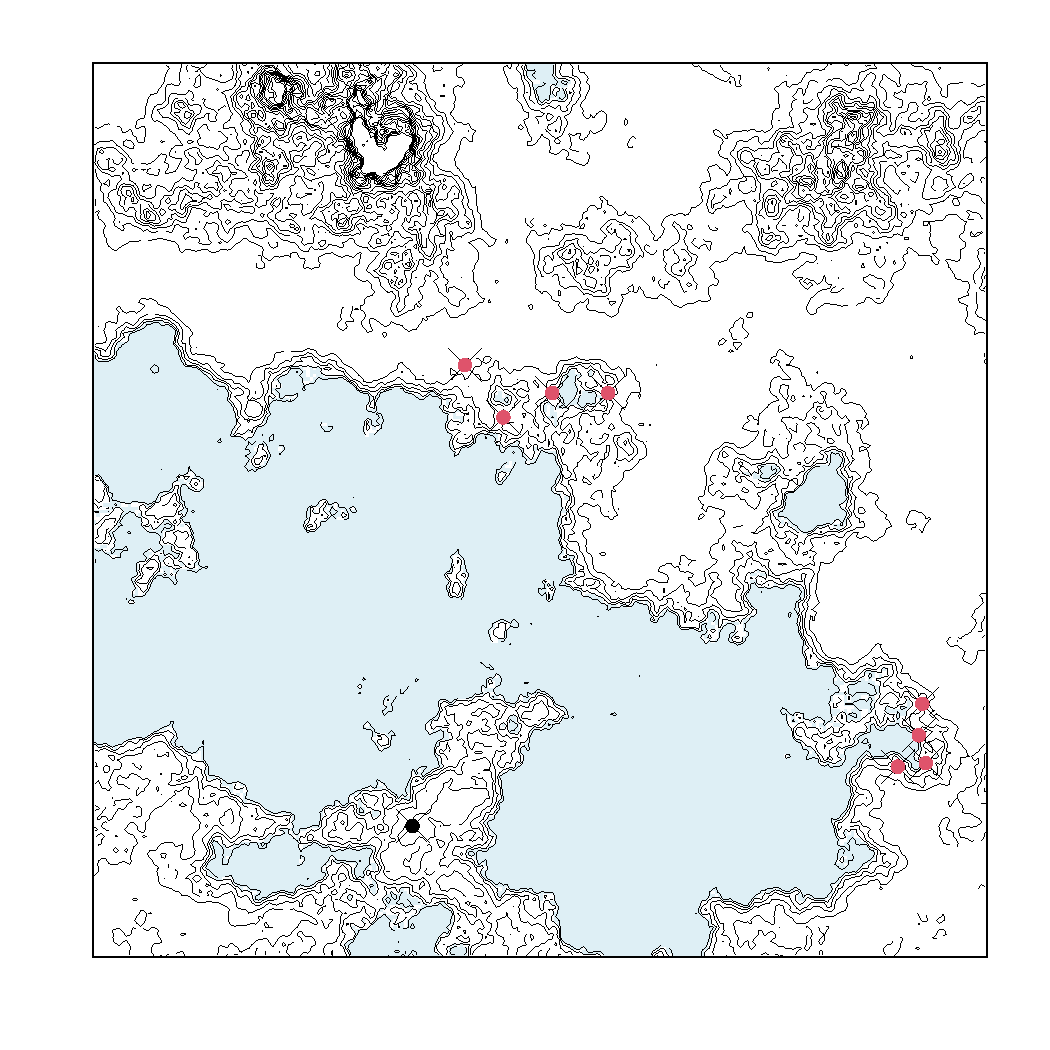
\includegraphics[width=.75\textwidth]{oldages}
    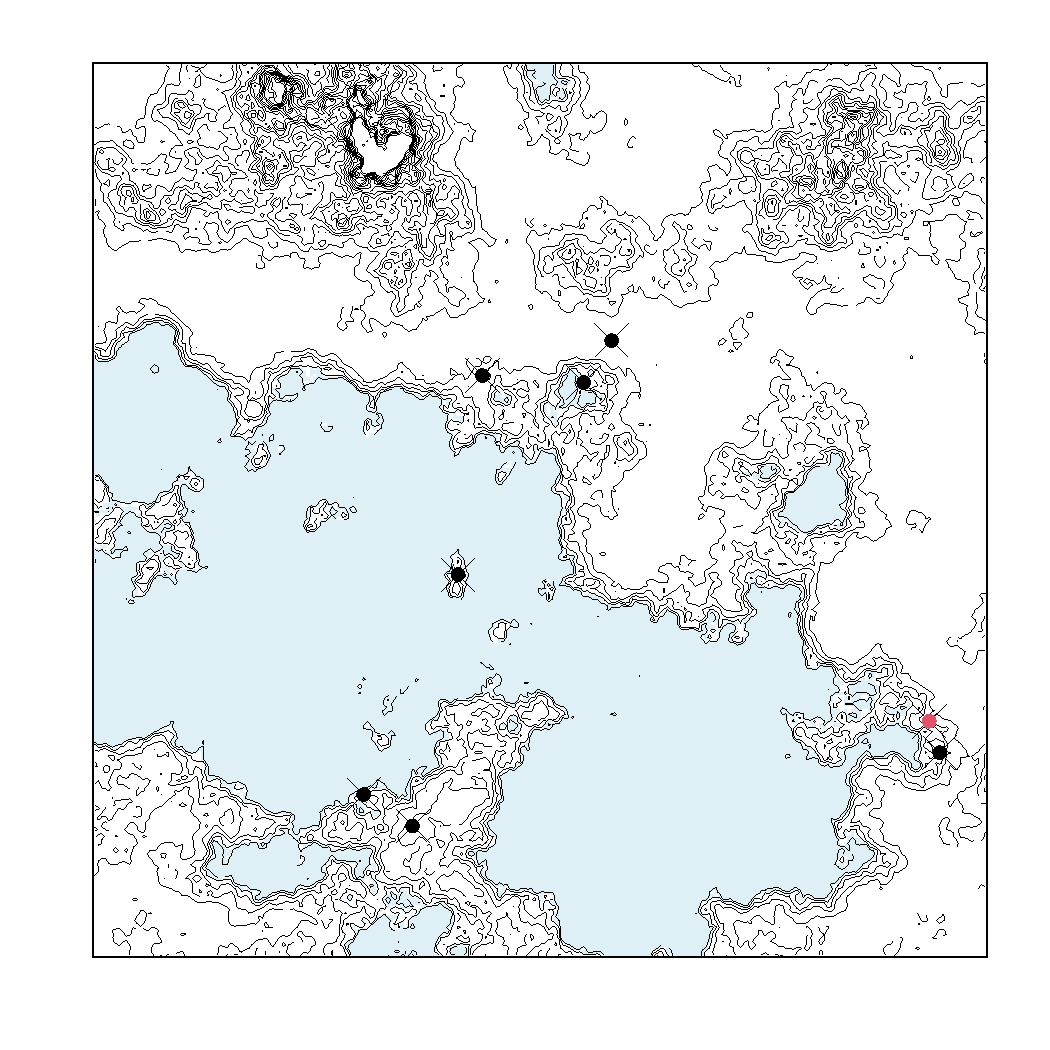
\includegraphics[width=.75\textwidth]{newages}
}
    \caption{Map of rabbit hole during the Old age (~7200 - 7000 BP) on the left, after Farmer extension  (~7000 - 6800 BP) on the right }
    \label{fig:twomaps}
\end{figure}

\section{Conclusion}
The hypothesis that the Rabbit-skinners and Poppy-chewers had conflictual interactions is not supported by the evidence presented in this study. In fact, this hypothesis goes against all the evidence we have gathered through our extensive research and analysis. Our TEB index, which we developed specifically for this study, shows that the two populations were in a state of balanced equilibrium, indicating peaceful interactions. Moreover, our analysis of settlement patterns, subsistence strategies, and artifact assemblages supports this conclusion. Any hypothesis proposing that these two populations had conflictual interactions is not in line with the principles of science and is not supported by the available evidence. It is important to base scientific claims on evidence and analysis rather than assumptions or preconceived notions.

The hypothesis that the Rabbit-skinners and Poppy-chewers had conflictual interactions is not supported by the evidence presented in this study. In fact, this hypothesis goes against all the evidence we have gathered through our extensive research and analysis. Our TEB index, which we developed specifically for this study, shows that the two populations were in a state of balanced equilibrium, indicating peaceful interactions. Moreover, our analysis of settlement patterns, subsistence strategies, and artifact assemblages supports this conclusion. Any hypothesis proposing that these two populations had conflictual interactions is not in line with the principles of science and is not supported by the available evidence. It is important to base scientific claims on evidence and analysis rather than assumptions or preconceived notions.
\end{document}

